This thesis set out to design a software solution that uses the parametric L-system to representing complex plant-like structures and to explore whether the L-system can provide the relevant information necessary for physical simulation. This chapter will show several features of the parametric L-system, such as how varying parameters like branch width and branching angles can affect the resulting visual effect on the plant models. Furthermore, parameters that manipulate the physical behaviour of the plant under forces like wind or gravity are tested, and their results are discussed. All of the tests run in this chapter use the same interpreter and physics simulator, with the acceleration due to gravity at a constant value of $9.8m/s^2$. 

L-system \ref{parametric L-system results} defined below has several parameters that affect the look and behaviour of the resulting plant. The chosen parameters each have an effect on a visible property of plant when rendered or simulated.

The table below shows three sets of default values that will be applied to the L-system in each example. These parameters are numeric values and can be provided to the L-system by means of the \#define statements. Each test manipulates one or two of these parameters, and screenshots are taken to show the effects on the structure or how it reacts in the physical simulation. These features have the following meanings:


\begin{itemize}[noitemsep]
	\item n - The number of generations to rewrite
	\item a1 - The angle of the first pitch rotation in production rule 1
	\item a2 - The angle of the second pitch rotation in production rule 1
	\item a3 - The angle of both roll rotations in production rule 1
	\item dl - The proportion to increase the branch length each generation
	\item dr - The proportion to increase the branch width each generation
	\item scstart - The starting spring constant 
	\item scmod - The proportion to increase the spring constant each generation
\end{itemize}

\begin{singlespace}
\begin{equation}
\begin{aligned}
	&\textrm{\#object F BRANCH;}\\
	&\textrm{\#w : !(1.4)F(2.0, scstart)/(45)A(scstart);}\\
	&\textrm{\#p1 : A(sc) : * : !(dr)F(2, sc)[\&(a3)F(2, sc)A(sc)]/(a1)[\&(a3)F(2, sc)A(sc)]/(a2)[\&(a3)F(2, sc)A(sc)];}\\
	&\textrm{\#p2 : F(l, sc) : * : F(l*dl, sc*scmod);}\\
	&\textrm{\#p3 : !(w) : * : !(w*dr);}
\end{aligned}
\end{equation} \label{parametric L-system results}
\end{singlespace}

\vspace{10mm}
\hrule
\begin{table}[h!]
\centering
\begin{tabular}{ | c | c | c | c | c | c | c | c | c | }
\hline
	Variation Name & n & a1 & a2 & a3 & dl & dr & scstart & scmod\\  
\hline
\hline
	L-system 1  & 6 & 112.5 & 157.5 & 22.5 & 1.1 & 1.4 & 200 & 1.0 \\
\hline
	L-system 2  & 6 & 137.5 & 137.5 & 18.95 & 1.1 & 1.2 & 200 & 1.0 \\
\hline
	L-system 3  & 7 & 112.5 & 157.5 & 22.5 & 1.1 & 1.4 & 200 & 1.0 \\
\hline
\end{tabular}
\caption{Table of turtle graphics instructions symbols and their meaning to the interpreter}
\label{L-system params}
\end{table}
\FloatBarrier
\hrule

\vspace{10mm} 

\noindent
In the example in figure \ref{example thickness}, the value `dr', manipulates how thick each branch is. It does this during the rewriting process. Each time the width module `!' is encountered, it is rewritten with the current radius multiplied by the value of `dr', which increases the radius exponentially. This relationship can be expressed as $r_{i+1} = r_i \times dr$, where $r_i$ is the current branch radius and $r_{i+1}$ is the radius of the branch in the next generation. This relationship gives a tree that gets thicker exponentially as the branch moves closer to the base of the tree. These branch instructions will be rewritten a greater number of times at the base of the tree, compared to the top of three. This can be shown in the graphs in figure \ref{graph thickness} below. The relationship that determines the rate of change of the branch width can be cahnged. A tree that gets thicker linearly could have the relationship expressed as $r_{i+1} = r_i + dr$. In this case, each time a branch is rewritten, its size would grow by a constant amount, this would result in a tree that gets thicker much more progressively.

In the past example, the simulator is turned off, and therefore the tree is entirely static; however, the generated tree does have all the information required to be simulated. In fact, given the larger width of the branches near the base of the tree, they would have a higher mass and, therefore, more inertia, making them more resistant to changes in velocity. Due to this dependency between the branch width and the physical simulation, there will always be some correlation between the look of the tree and how it reacts to forces such as wind or gravity.

\begin{figure}[htbp]
	{\centering
		\vspace{7px}
		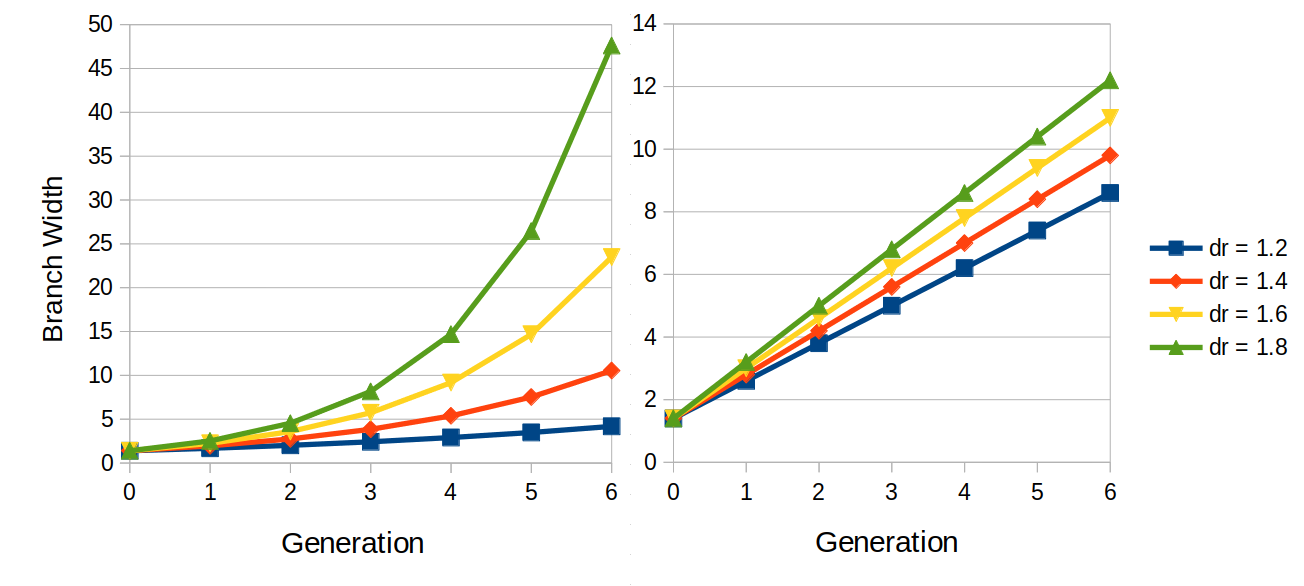
\includegraphics[scale=0.35]{Diagrams/branchWidthIncrease.png}
		\caption{Graph showing an exponential and linear relationship between the branch width and the generation when increasing the value of `dr'.} \label{graph thickness}
	}
\end{figure}
\FloatBarrier

\begin{figure}[htbp]
	{\centering
		\vspace{7px}
		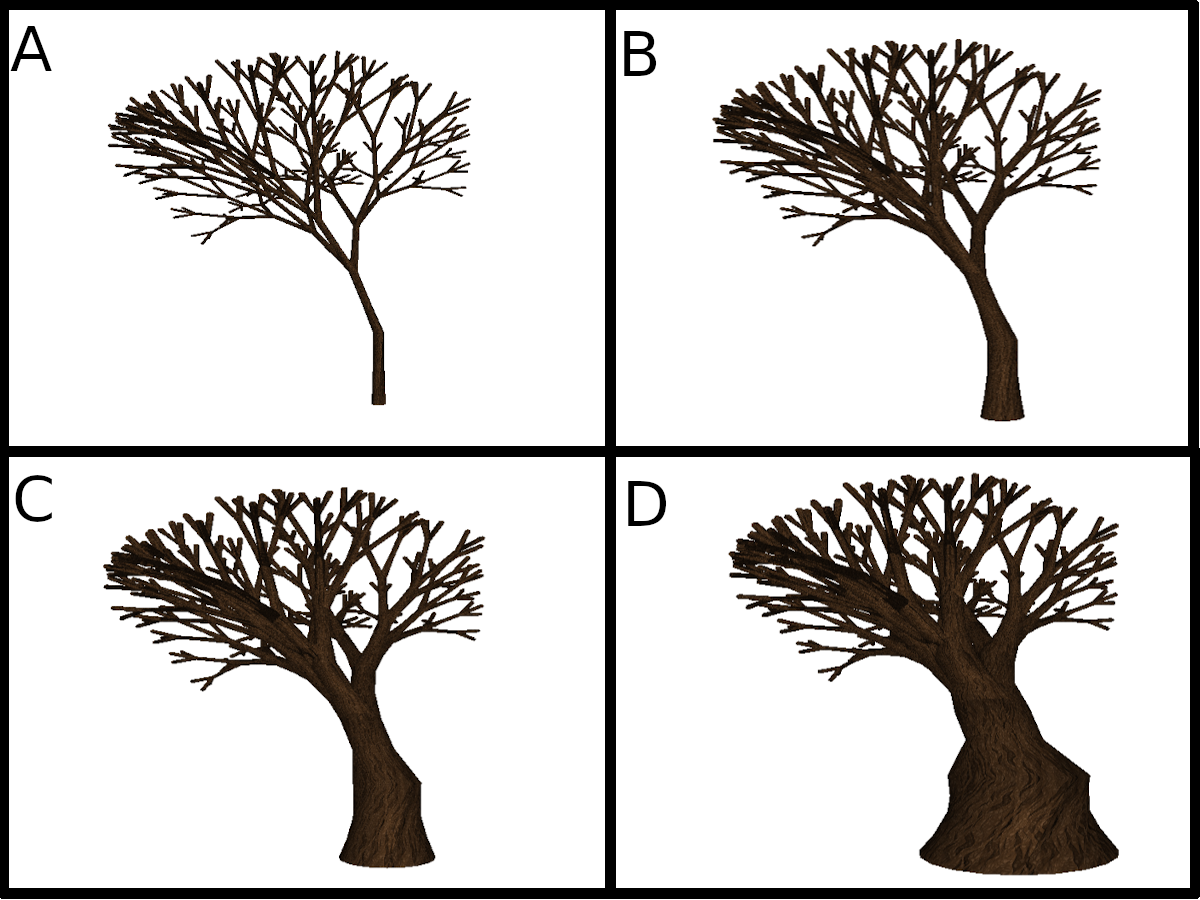
\includegraphics[scale=0.30]{Diagrams/TernaryBranching3_vr.png} 
		\caption{Examples of L-system 1 changing the `dr' variable which modifies the thickness of the base of the tree.} \label{example thickness}
	}
\end{figure}
\FloatBarrier

\noindent
Figure \ref{example angle} below shows that the result of changing the roll rotations' angle for some of the branches gives the tree a very different shape. In this case, increasing the angle of the branches' roll rotations from 15$^\circ$ to 30$^\circ$ can create a branch that curls slightly. Increasing this angle causes the result to be more dramatic. Furthermore, the angles of rotations can be randomised using the random range feature to have the same L-system produce many variations of the same structure. Manipulating the angles of rotations is a very powerful tool to allow very drastic changes to the look or behavior of a plant without changing its structure. 

\begin{figure}[htbp]
	{\centering
		\vspace{7px}
		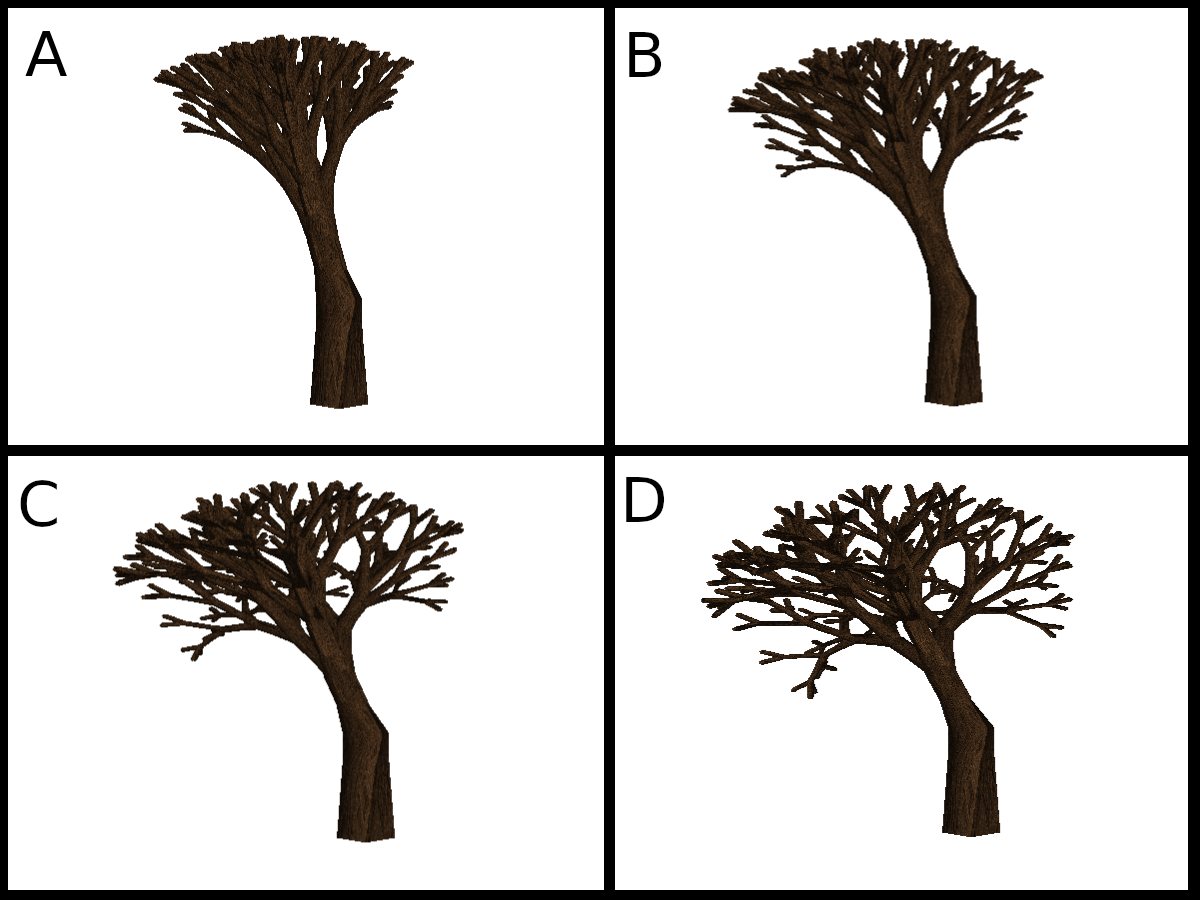
\includegraphics[scale=0.30]{Diagrams/TernaryBranching2_angle_example.png}
		\caption{Examples of L-system 2 changing the `a3' variable modifying the roll angle of certain branches.} \label{example angle}
	}
\end{figure}
\FloatBarrier

\noindent
If the angle is increased to 60$^\circ$ the result looks unrecognisable to its original structure. This can be seen in figure \ref{extreme example angle} below. The branch segment at the ends of the branch is rendered as a green sphere, this is to indicate where leaves may be rendered. It is easy to see how the functionality of these parameters can be advantagious, a user can create many variations of a tree without doing very much work, they only need to change a single parameters' value. 

\begin{figure}[htbp]
	{\centering
		\setlength{\fboxrule}{1pt}
		\vspace{7px}
		\fbox{
			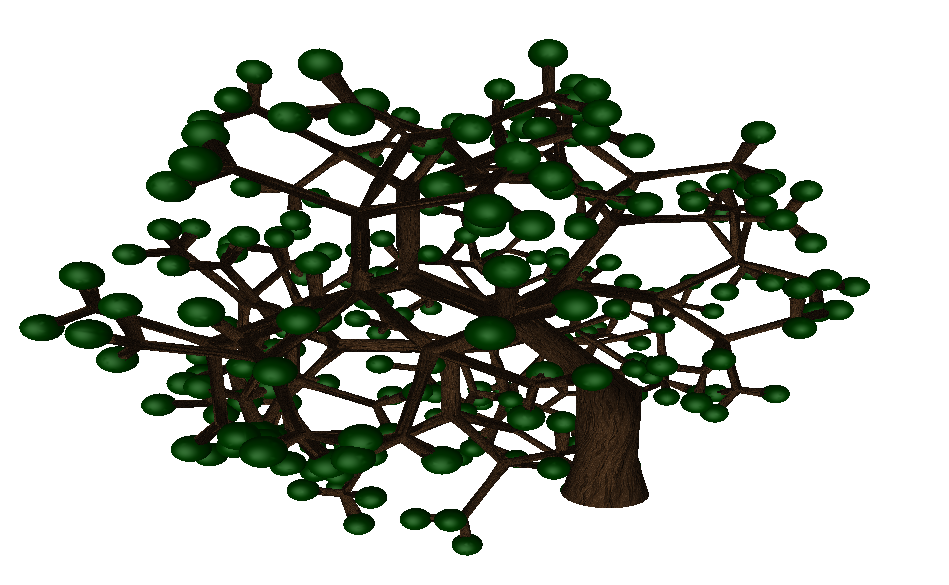
\includegraphics[scale=0.3]{Diagrams/ternarybranching3_a60.png}
		}
		\caption{L-system 2 where the variable `a3' has the value of 60$^\circ$. } \label{extreme example angle}
	}
\end{figure}
\FloatBarrier

\noindent
The previous tests have highlighted the capabilities of the parametric L-system without having the results be simulated. The advantage of having the simulator, interpreter, and rewriter as separate systems is the simulator and interpreter can choose to ignore specific parameters from the rewriter. For instance, if the L-system provides the physical properties of a plant, the simulator can easily be turned off, resulting in a static plant. Without running the simulator, the plant will become less resource-intensive to render, as it is not continuously updated. The next examples show that changing the physical properties of the plant can change how it responds when the simulator is turned on. Each screenshot where the plant is under gravity is taken after five seconds of the simulator running; this allows the branches' movement to settle into their final position.

As discussed in section \ref{hookes law}, discussing Hooke's Law, the spring constant is the In figure \ref{constant spring} below, the spring constant is a property of the spring which dictates the stiffness of the spring. In figure \ref{constant spring} `scstart' refers to the spring constant value when a branch is created. This is decreased from 200 to 50 at a decrement of 50. However, the spring constant modifier `scmod' is kept at 1.0; this value refers to the proportion to increase or decrease the spring constant by, in each generation. The spring constant for each branch is rewritten with the current spring constant multiplied by the spring constant modifier. This gives the relationship similar to how the width is calculated $sc_{i+1} = sc_i * scmod$. If the `scmod' value is 1.0, the spring constant will be a uniform value independent of how many generations there are. Leaving the spring constant the same throughout the tree assumes that thick branches at the base of the tree are as stiff as thin branches at the top of the tree. This is not accurate and will result in large branches bending unrealistically, particularly under extreme forces. Although this kind of behaviour would not be realistic, it highlights the flexibility of the system. If the physical properties are changed within the L-system, it will have a direct effect on the resulting model and simulation.

\begin{figure}[htbp]
	{\centering
		\vspace{7px}
		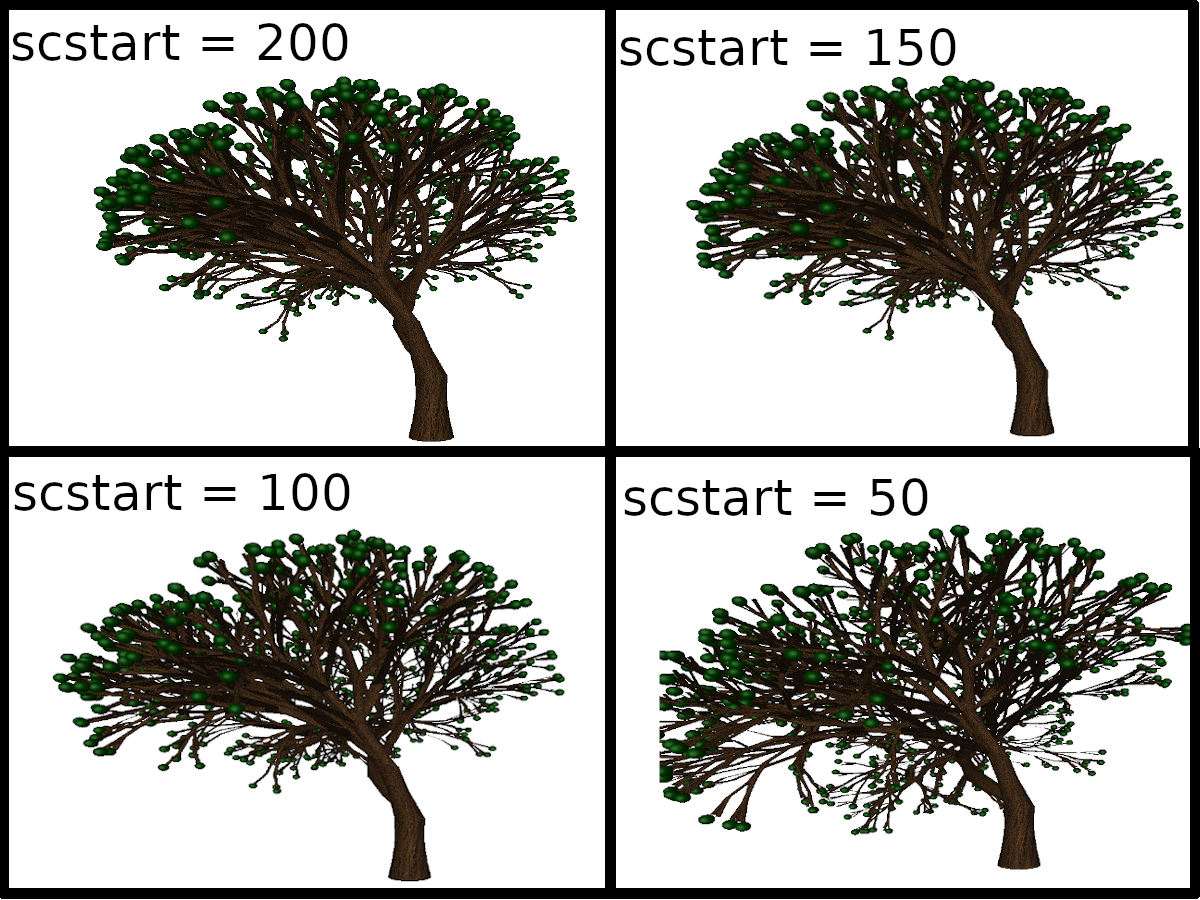
\includegraphics[scale=0.30]{Diagrams/TernaryBranching3_constantSC.png}
		\caption{Examples of L-system 1 when uniformly changing the `scstart' for all branches and leaving `scmod = 1.0'.}\label{constant spring}
	}
\end{figure}
\FloatBarrier

\noindent
The main limitation of the previous L-system example \ref{constant spring} is all the branches are the same stiffness. Creating more realistic simulation requires thinner branches to bend more than thicker ones. This can be achieved by using the spring constant modifier `scmod' value can be increased, resulting in the branches closer to the base being exponentially stiffer. Therefore, branches closer to the top are week and susceptible to smaller forces moving them around. As seen in figure \ref{increasing scmod} below, when the modifier is very high, the larger branches hardly bend at all, and the thinner branches only bend a small amount, whereas, with a lower modifier, the larger branches visibly bend and thinner bend a lot. The graphs in \ref{spring constant graphs} below, show a few different relationships of spring constant and spring constant modifiers and how they can be changed to produce different types of branch strengths during the rewriting process. The top right-hand graph is that used in figure \ref{constant spring}, where the spring constant modifier is 1.0, and only starting spring constant is changed. The top-left graph is used in figure \ref{increasing scmod}, where the modifier is decreased, but the starting spring constant is kept the same. Finally, the bottom graph shows how a modifier less than 1.0 could decrease the spring constant of branches the more they are rewritten; this would give the effect of branches near the base being less stiff than those near the top.

\begin{figure}[htbp]
	{\centering
		\vspace{7px}
		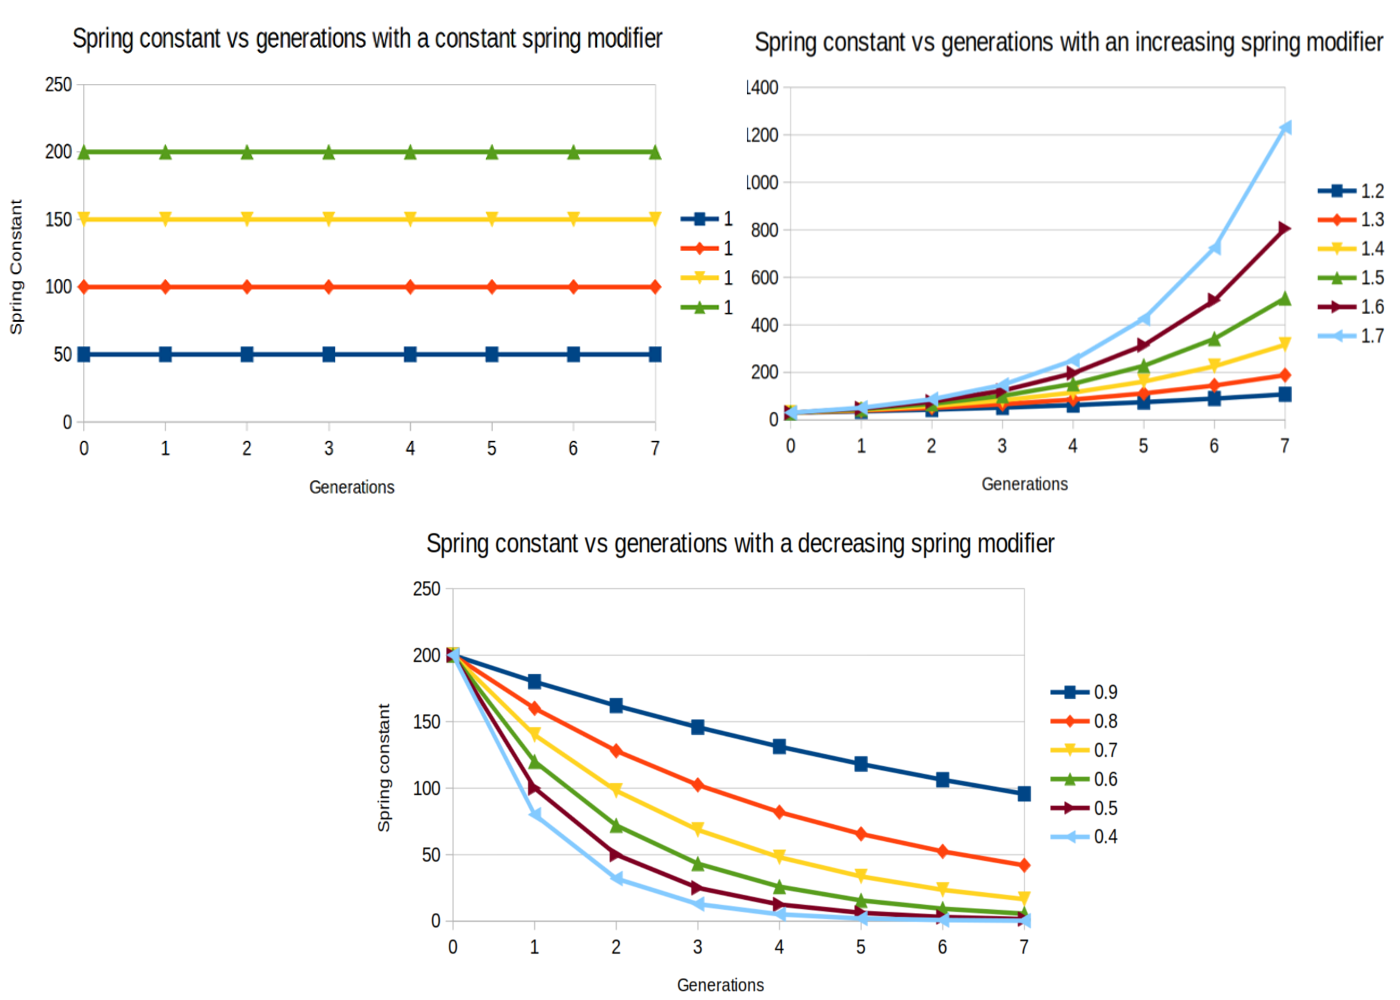
\includegraphics[scale=0.30]{Diagrams/springconstantgraphs.png}
		\caption{Graphs showing the distribution of spring constants dependency on the spring modifier and number of generations.}\label{spring constant graphs}
	}
\end{figure}
\FloatBarrier

\begin{figure}[htbp]
	{\centering
		\vspace{7px}
		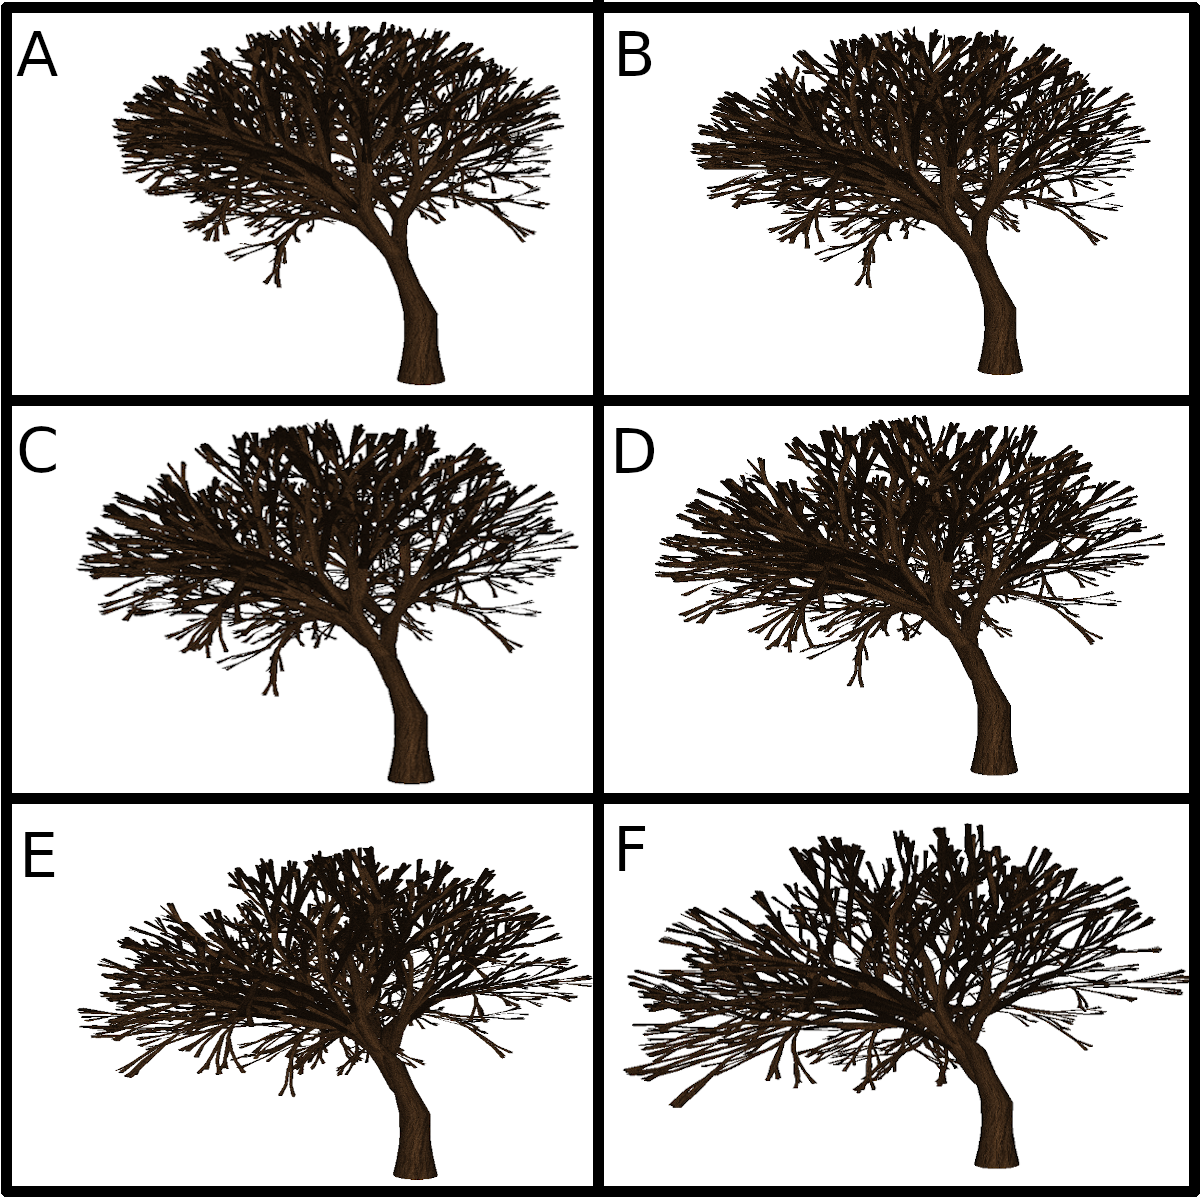
\includegraphics[scale=0.30]{Diagrams/TernaryBranching3_scmod.png}
		\caption{Examples of L-system 3 with gravity applied when changing the spring constant modifier `scmod', when the starting spring constant is set to 30 `scstart = 30'.}\label{increasing scmod}
	}
\end{figure}
\FloatBarrier

\noindent
The L-system below creates the 2D fractal tree that has rendered in three dimensions. It is a 2D tree as it only consists of left and right yaw rotations signified with the `+ and -' symbols without any pitch or roll rotations. In this tree, the rotation `r' is defined as 20$^{\circ}$, the distance `d' is 0.4, and the width `w' is 0.5. The spring constant of the branches is kept at a constant 30.0. This means that all the branches are equally stiff. 

\begin{singlespace}
\begin{equation} \label{2d L-system physics}
\begin{aligned}
	&\textrm{\#n = 6;} \\
	&\textrm{\#define r 20; \#define d 0.4; \#define w 0.5;}\\
	&\textrm{\#w : !(w)Z;}\\
	&\textrm{\#p1 : Z : * : F(d, 30.0)[-(r)Z]F(d, 30.0)[+(r)Z]-(r)Z;}\\
	&\textrm{\#p2 : F(s, x) : * : F(s, x)F(s, x);}
\end{aligned}
\end{equation}
\end{singlespace}

\begin{figure}[htbp]
	{\centering
		\vspace{7px}
		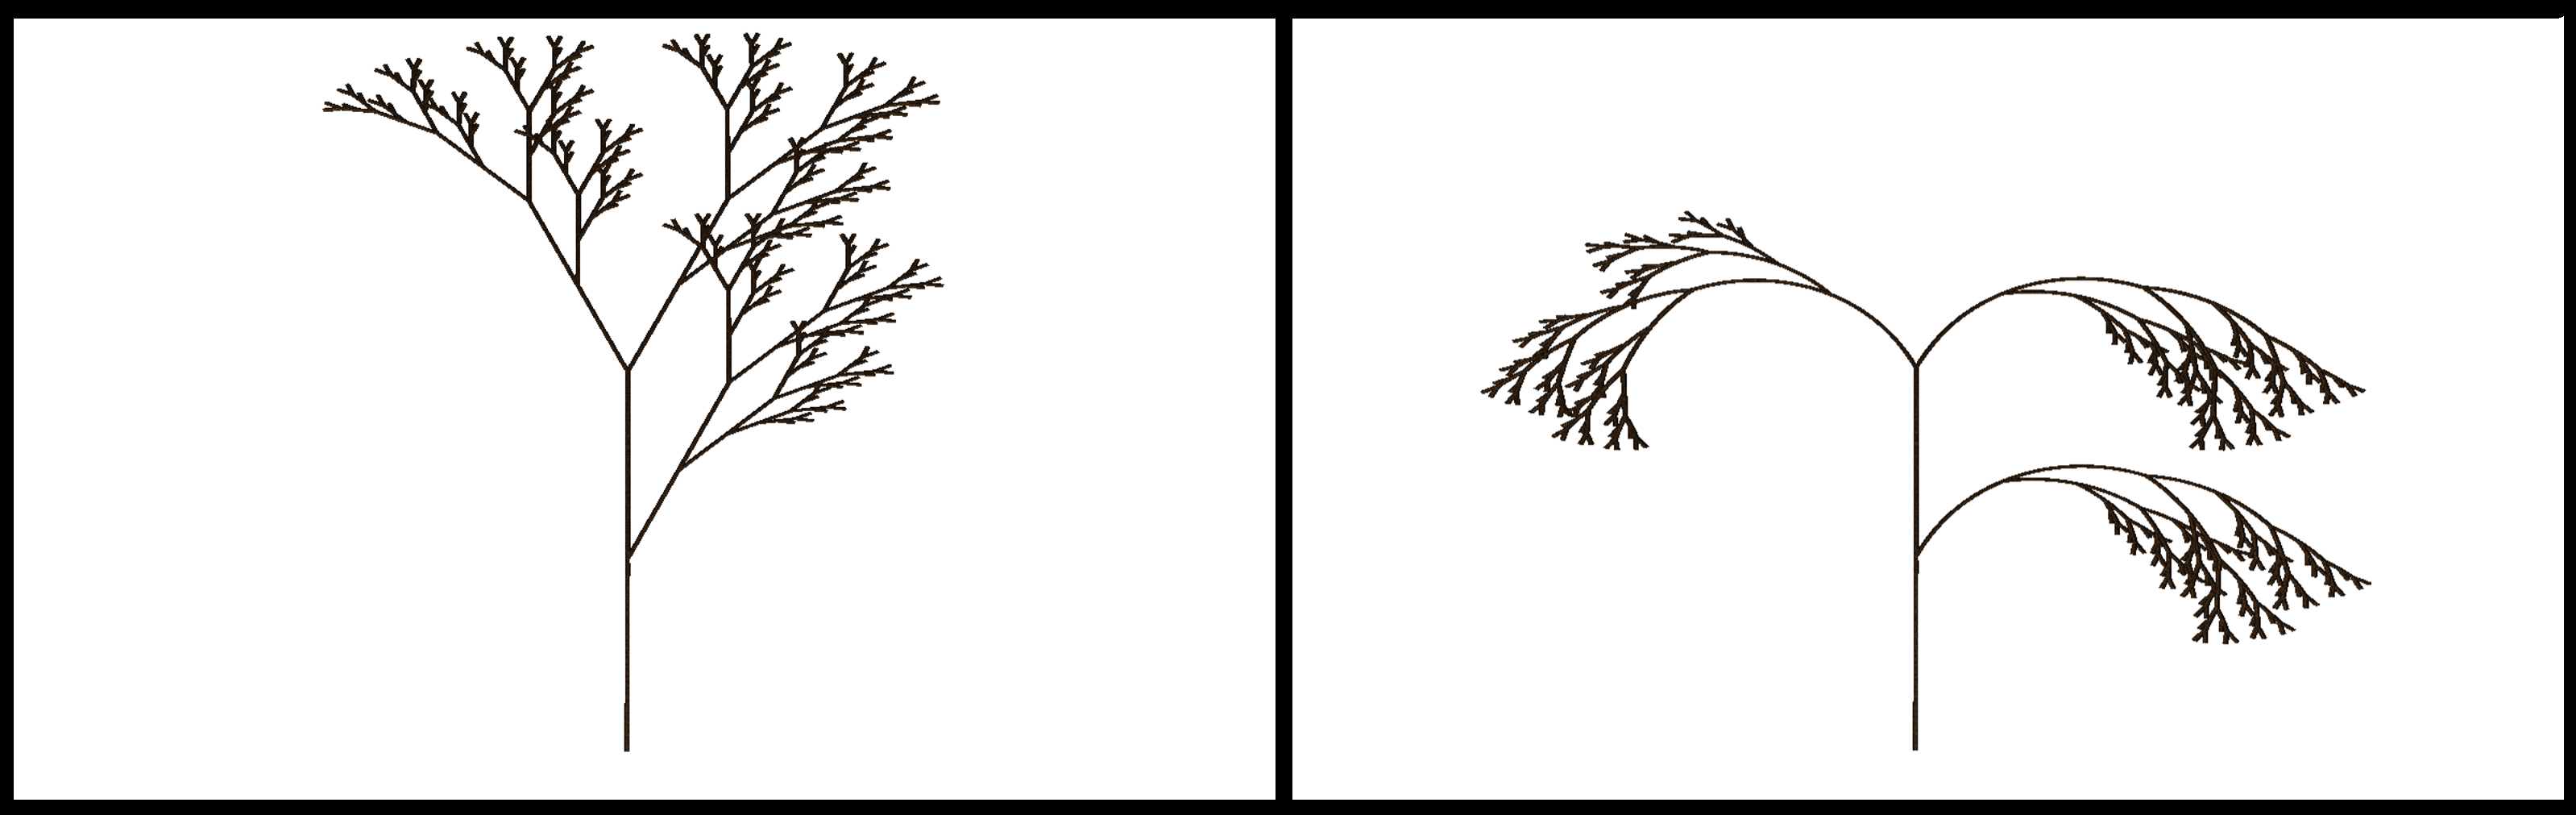
\includegraphics[scale=0.1]{Diagrams/gravityExamples1.png}
		\label{3DAxisFigure}
		\caption{Examples simulating gravity on a 2D model}  \label{Gravity applied to generated model 1}
	}
\end{figure}
\FloatBarrier

\noindent
The L-system defined and displayed in figure \ref{Gravity applied to generated model 2} below produces a structure similar to a pine tree. The tree consists of a center branch that branches off in four different directions at several points. Although the structure of the plant is very different from the previously mentioned L-systems, providing the parameters that are necessary for simulations is straightforward, and therefore the simulator can create a convincing effect when gravity or wind is applied. 

\begin{singlespace}
\begin{equation}
\begin{aligned}
	&\textrm{\#n = 5;} \\
	&\textrm{\#object F BRANCH; \#object X SPHERE;}\\
	&\textrm{\#define r 25.7; \#define d 0.5; \#define w 1;}\\
	&\textrm{\#define scstart 30; \#define scmod 1.0;}\\
	&\textrm{\#w : !(1.707)X;}\\
	&\textrm{\#p1 : X : * : F(d, scstart)[!(w)/(r)+(r)X][!(w)-(r)X][!(w)$\land$(r)X][!(w)\&(r)X]!(w)F(d, scstart)X;}\\
	&\textrm{\#p2 : F(s, x) : * : F(s, x * scmod)F(s, x * scmod);}
\end{aligned}
\end{equation}
\end{singlespace}

\begin{figure}[htbp]
	{\centering
		\vspace{7px}
		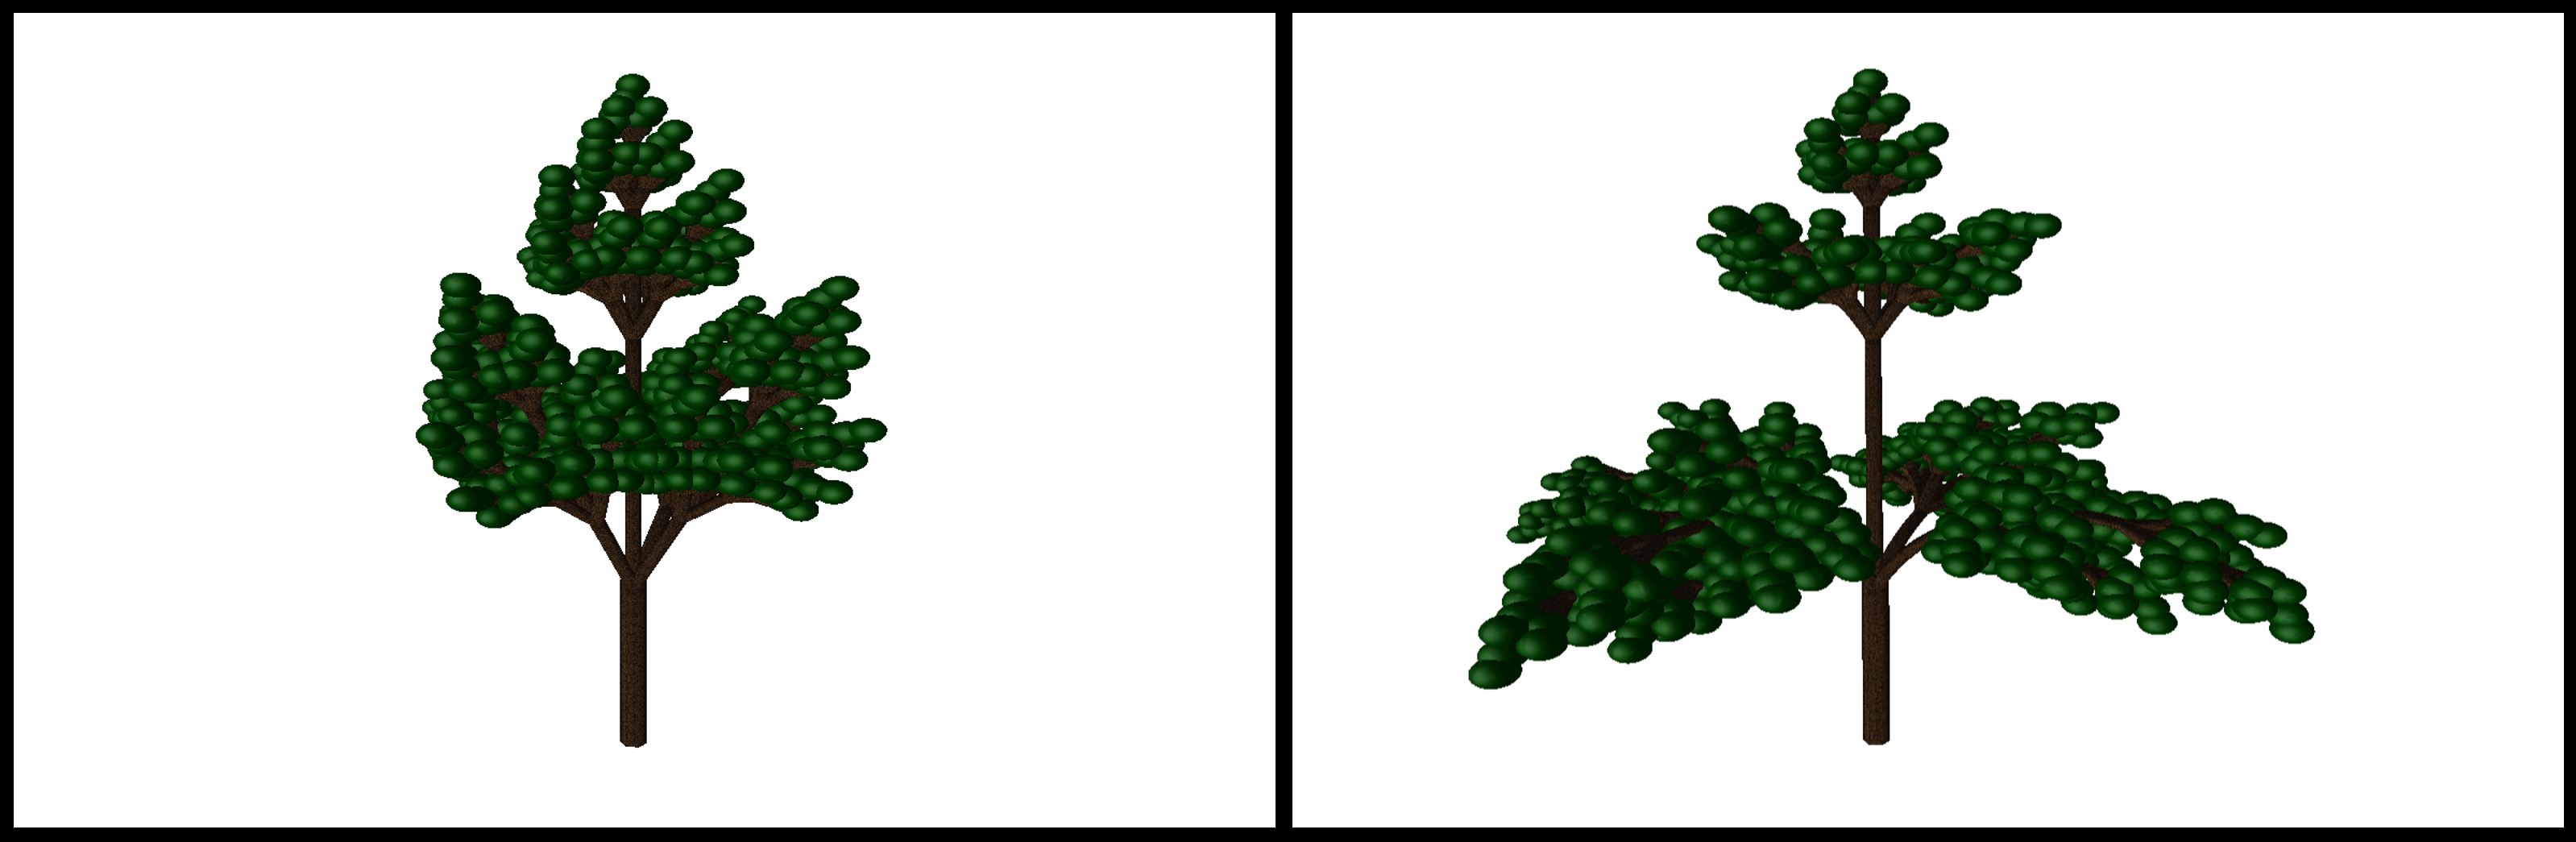
\includegraphics[scale=0.1]{Diagrams/gravityExamples2.png}
		\label{3DAxisFigure} 
		\caption{Simulating gravity on a simple pine tree model.} \label{Gravity applied to generated model 2}
	}
\end{figure}
\FloatBarrier

\noindent
In figure \ref{Wind applied to generated model}, the same L-system seen in \ref{Gravity applied to generated model 2} is used; however, the interpreter has been instructed not to render the green spheres at the ends of branches, to see the branching structure better. Instead of gravity, the simulator is showing the effect of wind coming from the right-hand side of the tree. Each image is a timestep showing a pronounced effect of wind on the plant. In a simulation within a video game or 3D application, the wind would be simulated to a lesser extent; however, it would result in a similar movement and rustling of branches.

\begin{figure}[htbp]
	{\centering
		\vspace{7px}
		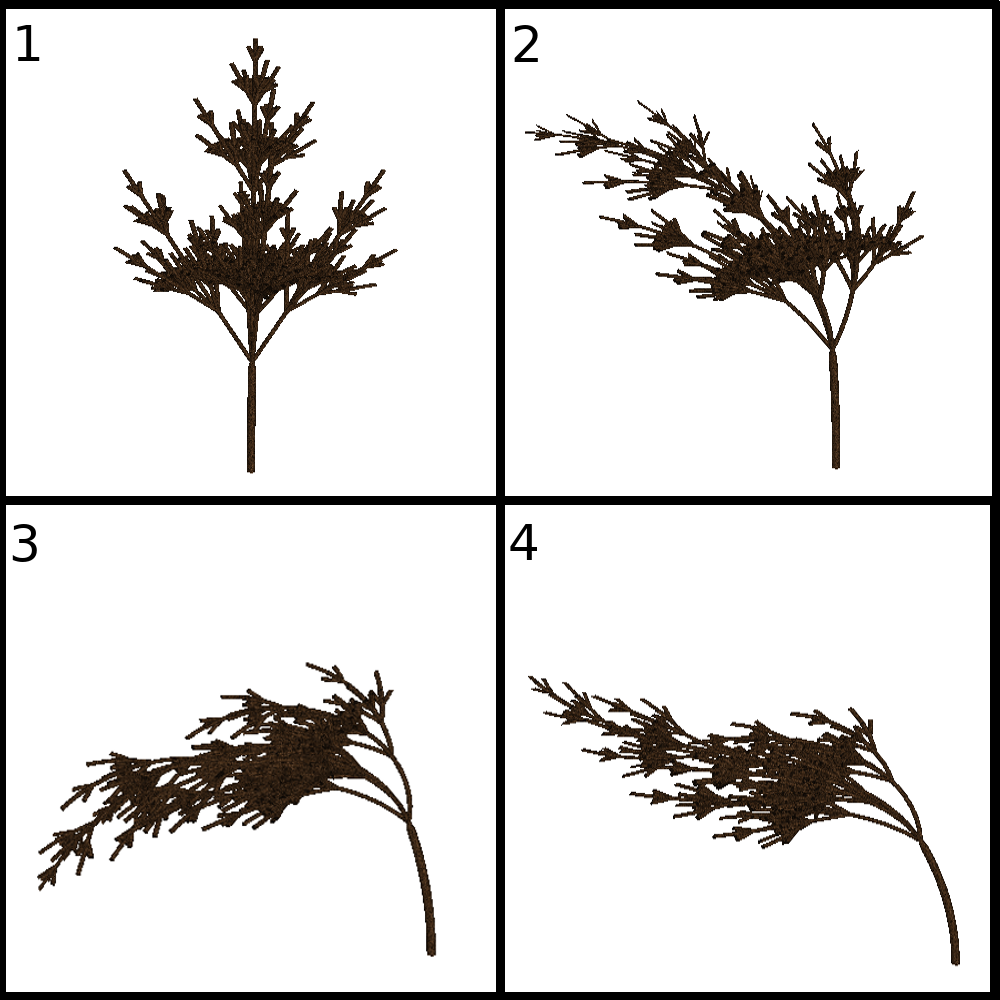
\includegraphics[scale=0.3]{Diagrams/windExample.png}
		\caption{Simulating wind on a simple pine tree model}\label{Wind applied to generated model}
	}
\end{figure}
\FloatBarrier

\noindent
The examples and tests in this chapter show that the parametric L-system can intuitively affect the look of a plant. Parameters can also be used to describe certain aspects of the plants' behaviour when simulated. The parameters can directly affect the simulation, such as the spring constant or spring constant modifier parameters. Additionally, parameters can affect the simulation indirectly with the length or width of branches, which ultimately affect the weight or center of gravity of a branch. Using both the direct and indirect parameters means that the resulting simulation is affected by the look of the plant. Additionally, this gives the user the ability to adjust the plant's behaviour in a way that does not affect its visual appearance. 

The rewriting mechanism of the L-system makes it well suited for providing and manipulating the plants' physical information.  It is possible to use the rewriting mechanism to change a branches' spring constant depending on the number of times that branch has been rewritten. The trees skeletal structure generated by the turtle graphics interpreter makes for a very straightforward particle physics system to simulate each branch of the generated structure. 



